\documentclass[twoside,11pt]{article}

\usepackage[utf8]{inputenc}
\usepackage[T1]{fontenc}
\usepackage[ngerman]{babel}
\usepackage{graphicx,curves,float,rotating}
\usepackage[usenames,dvipsnames,svgnames,table]{xcolor}
\usepackage{latexsym,amsmath,amssymb}
\usepackage{a4,amsmath}
\usepackage{theorem}
\usepackage{dcolumn}
\usepackage{fancyhdr}
\usepackage{extramarks}
\usepackage{sectsty}
\usepackage[light]{roboto}

\newcommand{\Frac}[2]{\frac{\displaystyle #1}{\displaystyle #2}}
\newlength{\textwd}
\newlength{\oddsidemargintmp}
\newlength{\evensidemargintmp}
\newcommand{\hspaceof}[2]{\settowidth{\textwd}{#1}\mbox{\hspace{#2\textwd}}}
\newlength{\textht}
\newcommand{\vspaceof}[3]{\settoheight{\textht}{#1}\mbox{\raisebox{#2\textht}{#3}}}
\newcommand{\PreserveBackslash}[1]{\let\temp=\\#1\let\\=\temp}

\newenvironment{deflist}[1][\quad]%
{  \begin{list}{}{%
	\renewcommand{\makelabel}[1]{\textbf{##1}\hfil}%
	\settowidth{\labelwidth}{\textbf{#1}}%
	\setlength{\leftmargin}{\labelwidth}
	\addtolength{\leftmargin}{\labelsep}}}
{  \end{list}}

\newenvironment{Quote}% Definition of Quote
{  \begin{list}{}{%
	\setlength{\rightmargin}{0pt}}
	\item[]\ignorespaces}
{\unskip\end{list}}

\newtheorem{Cor}{Corollary}
\theoremstyle{break}
\theorembodyfont{\itshape}
\newtheorem{Def}[Cor]{Definition}
\theoremheaderfont{\scshape}

\newcolumntype{.}{D{.}{.}{-1}}

\textwidth 15cm
\textheight 23cm
\oddsidemargin 1cm
\evensidemargin 0cm

% Colors:
\definecolor{blau}{HTML}{355FB3}

%Fonts:
\renewcommand{\rmdefault}{ppl}
\sectionfont{\sffamily\mdseries\textrmlf\LARGE\color{blau}}

% Header:
\fancyhf{}
\fancyhead[EL,OR]{\sffamily{\thepage}}
\fancyhead[OL,ER]{\nouppercase{\sffamily{\firstleftmark}}}

\begin{document}

% Titelseite:
\pagestyle{empty}

\begin{center}
	\sffamily
    Universität Paderborn \\
    Institut für Informatik \\
    Prof.\ Dr.\ Stefan Böttcher\\[2ex]
    Proseminar Datenkompression im WS 2016/2017

	\vspace*{\fill}
	\Huge \textcolor{blau}{Linear-Time Suffix-Sorting} \\[2ex]
    \LARGE Clemens Damke \\[1ex]
    \Large Matrikelnummer 7011488
	\vspace*{\fill}
\end{center}

\newpage
\
\newpage

% Inhaltsverzeichnis:
\pagestyle{fancy}
\tableofcontents

\newpage
\pagestyle{empty}
\
\newpage
\pagestyle{fancy}

\section{Problemstellung}
\label{sec:Problemstellung}

Diese Proseminar-Arbeit beschreibt den GSACA-Algorithmus. Hierbei handelt es sich um einen rekursionsfreien Linearzeitalgorithmus zur Konstruktion von Suffix-Arrays.
\\

Im Folgenden wird zunächst erörtert, was Suffix-Arrays sind und wozu sie benutzt werden.

\subsection{Was ist ein Suffix-Array?}

Das Suffix-Array $SA$ einer Zeichenkette $S$ ist definiert als die lexiographisch aufsteigend sortierte Folge aller Suffixe von $S$.

\begin{figure}[h]
	\centering
	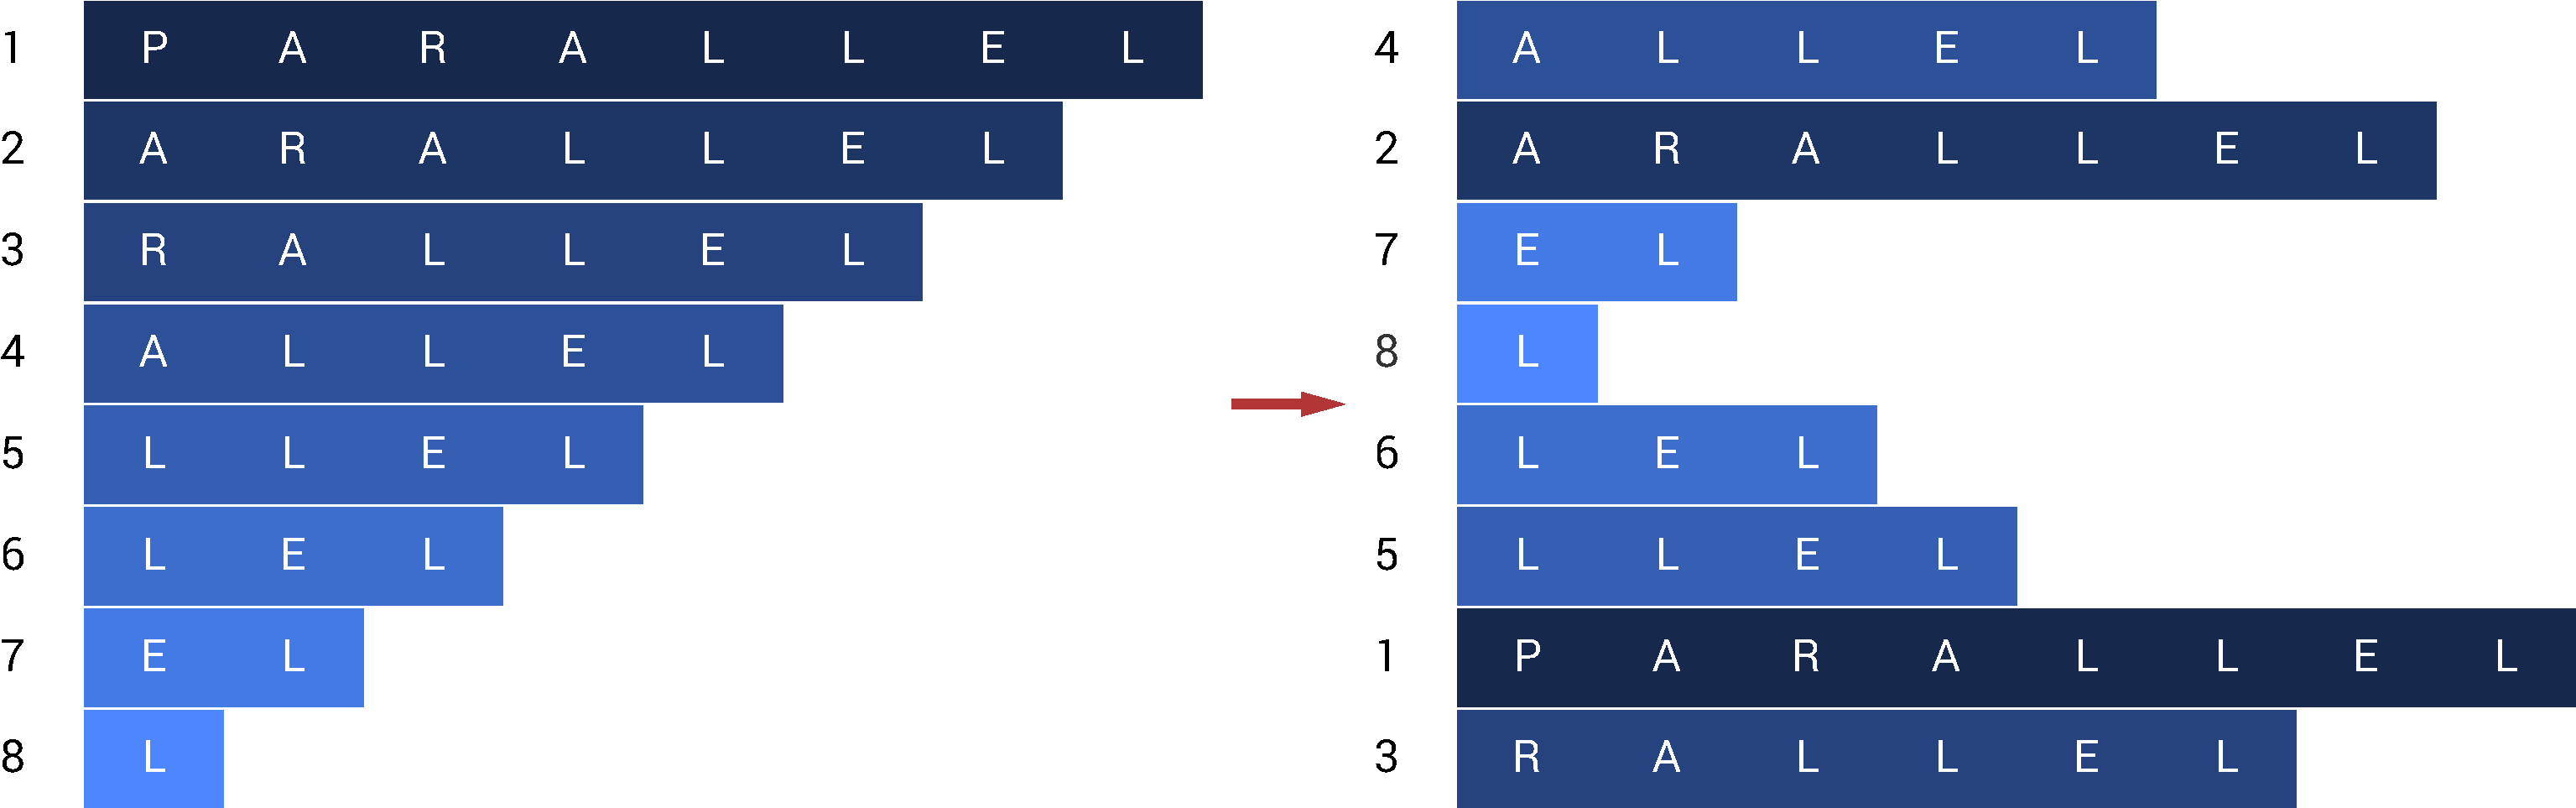
\includegraphics[width=\linewidth,bb=0 0 1474 462]{./assets/whatIsASuffixArray.pdf}
	\caption{Beispielhaftes Suffixarray mit $S =$ `parallel`}
\label{fig:whatIsASuffixArray}
\end{figure}

\subsection{Einsatzgebiete von Suffix-Arrays}

\section{Ansätze zur Suffix-Array-Konstruktion}

\subsection{Unterabschnitt}

\subsubsection{Unter-Unterabschnitt: Beispiel f\"ur Tabellen}

\begin{table}[H]
\begin{center}
\caption{Beispiel Tabelle}
\label{tab:beispiel}

\vspace{2ex}

\begin{tabular}{|l|c|r|}
\hline
links		&	zentriert	&	rechts  \\ \hline\hline
links2		&	zentriert2	&	rechts2 \\ \hline
XXXXXXXXXXX	& XXXXXXXXXXXXXXXXXXXXX	& XXXXXXXXXXXX  \\ \hline

\end{tabular}
\end{center}
\end{table}


\subsection{Unterabschnitt: Beispiel f\"ur Grafiken}

\section{Der GSACA-Algorithmus}

test

\section{Performanceanalyse}

test

\section{Fazit}

test

\newpage

\addcontentsline{toc}{section}{Literaturverzeichnis}
\bibliographystyle{plain}
\bibliography{paper}

\end{document}
